\Chapter{Megvalósítás}

\Section{A kód}
\SubSection{Kezdetek}
A legelején egy egyszerű python applikációba szerettem volna megvalósítani a megjelenítést és magát az egész projektet. Ehhez a TKInter nevű könyvtárat szándékoztam használni, állítható értékekkel, hogy megfigyeljem melyik érték kombinációval a legcélszerűbb a kép beolvasása és az adatok kinyerése onnan. Leegyszerűsített használatra, csak a sima akkordokkal foglalkozva ugye a kék színű akkordokat szándékoztam kinyerni a képből. Végül a csúszkákat félretéve manuálisan írtam át az értékeket, egy numpy (python függvénykönyvtár, többnyire tömbkezeléssel kapcsolatos) tömbbe csomagoltam be ezeket. Ezek az értékek kellettek ahhoz, hogy meghatározzam a cv2-nek, hogy milyen színskálába szeretném kiszedni az akkordokat. 
\par
Kísérleteztem azzal, hogy ha változtatom a skálát, akkor milyen pontossággal tudja visszaadni csak az akkordokat(amik kékkel vannak feltüntetve) a képről. Az volt a terv, hogy akkor ez mint bemeneti kép lesz majd kiolvasva a képből az OCR segítségével. Ehhez az kellett, hogy a megfelelő spektrumba legyen a program színhatára, amit ki tud olvasni zajmentesen, mivel a kották egységes kék színnel vannak kezelve akkordok terén, ezért nem kell egyáltalán változó értékű tömböket használni a színskála belövéséhez.
\par

\SubSection{A végleges program}
A következőkben áttértem jupyter-notebookra, hogy lehessen szétbontani, és emészthetőbbé varázsolni a kódot

\begin{python}
this_img = cv2.imdecode(numpyarray, cv2.IMREAD_UNCHANGED)	
\end{python}

\begin{figure}[h]
	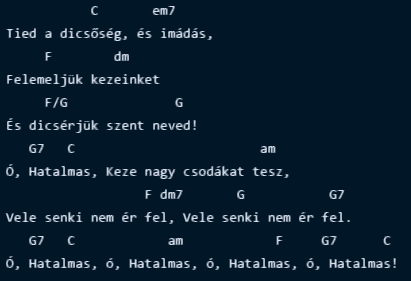
\includegraphics[scale=1]{images/output_tied.png}
	\caption{Az xml beolvasó program kimenete}
	\label{fig:output1}
\end{figure}

\begin{figure}[h]
	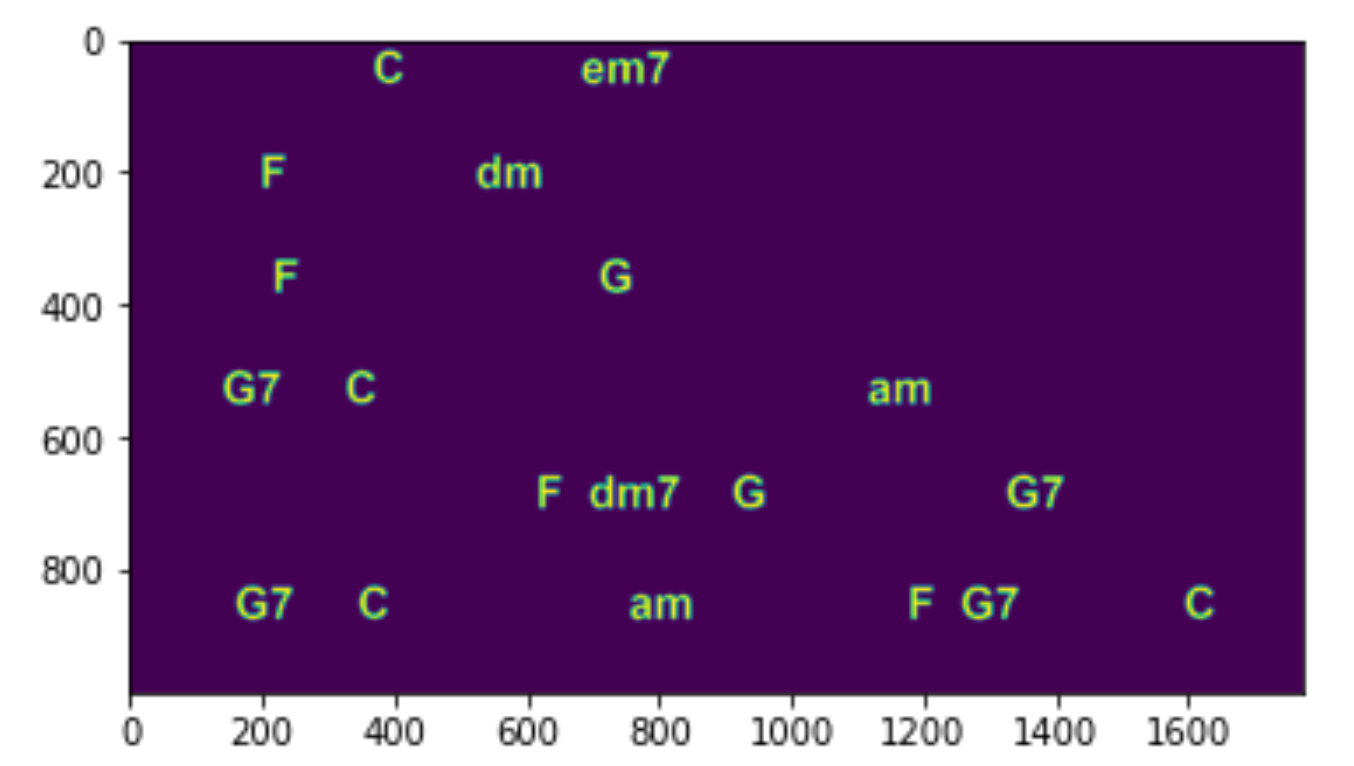
\includegraphics[scale=0.5]{images/output_justchords.png}
	\caption{Kotta akkordjai}
	\label{fig:output2}
\end{figure}

\begin{figure}[h]
	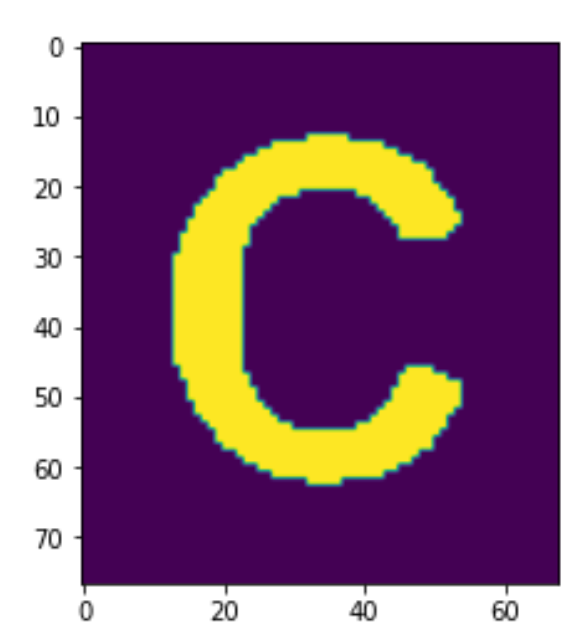
\includegraphics[scale=0.5]{images/output_single_character.png}
	\caption{A kotta egyik akkordja}
	\label{fig:output3}
\end{figure}